\chapter{\textbf{Программа по индивидуальному варианту}}
Задания выполнялись по варианту 16.

\section{\textbf{Задание №1}}
Создать новый файл, содержащий текст программы по индивидуальному варианту. Псевдокод, соответствующий данной программе, представлен на листинге \ref{lst:disassembler}.

\begin{lstlisting}[label=lst:disassembler,caption=Исходный текст исследуемой программы]
	.section .text
	.globl _start;
	len = 9;
	enroll = 1;
	elem_sz = 4;
	
_start:
	la x1, _x
	addi x20, x0, (len-1)/enroll
	lw x31, 0(x1)
	addi x1, x1, elem_sz*1
lp:
	lw x2, 0(x1)
	add x1, x1, elem_sz*enroll
	bltu x2, x31, lt
	add x31, x0, x2 #!
lt:
	addi x20, x20, -1
	bne x20, x0, lp
	lp2: j lp2
	
	.section .data
_x:     
	.4byte 0x1
	.4byte 0x2
	.4byte 0x3
	.4byte 0x4
	.4byte 0x8
	.4byte 0x6
	.4byte 0x7
	.4byte 0x5
	.4byte 0x4
\end{lstlisting}

Дизассемблированный код данной программы представлен на листинге \ref{lst:disassembler_code}.
\begin{lstlisting}[label=lst:disassembler_code,caption=Дизассемблированный код]
Disassembly of section .text:

80000000 <_start>:
80000000:       00000097            auipc   x1,0x0
80000004:       03008093            addi    x1,x1,48 # 80000030 <_x>
80000008:       00800a13            addi    x20,x0,8
8000000c:       0000af83            lw      x31,0(x1)
80000010:       00408093            addi    x1,x1,4

80000014 <lp>:
80000014:       0000a103            lw      x2,0(x1)
80000018:       00408093            addi    x1,x1,4
8000001c:       01f16463            bltu    x2,x31,80000024 <lt>
80000020:       00200fb3            add     x31,x0,x2

80000024 <lt>:
80000024:       fffa0a13            addi    x20,x20,-1
80000028:       fe0a16e3            bne     x20,x0,80000014 <lp>

8000002c <lp2>:
8000002c:       0000006f            jal     x0,8000002c <lp2>

Disassembly of section .data:

80000030 <_x>:
80000030:       0001                c.addi  x0,0
80000032:       0000                unimp
80000034:       0002                0x2
80000036:       0000                unimp
80000038:       00000003            lb      x0,0(x0) # 0 <enroll-0x1>
8000003c:       0004                c.addi4spn      x9,x2,0
8000003e:       0000                unimp
80000040:       0008                c.addi4spn      x10,x2,0
80000042:       0000                unimp
80000044:       0006                0x6
80000046:       0000                unimp
80000048:       00000007            0x7
8000004c:       0005                c.addi  x0,1
8000004e:       0000                unimp
80000050:       0004                c.addi4spn      x9,x2,0
\end{lstlisting}

Код, поясняющий работу данной программы представлен на листинге \ref{lst:pseudocode}.
\begin{lstlisting}[label=lst:pseudocode, caption=Дизассемблированный код]
#define len 9
#define enroll 1
#define elem_sz 4

int _x[] = {1,2,3,4,8,6,7,5,4};
void _start()
{
	int *x1 = _x;
	int x31 = x1[0];
	int x20 = (len - 1) / enroll;
	int x1 = elem_sz * 1;
	
	do
	{
		int x2 = x1[0];
		x1 += elem_sz * enroll;
		if (x2 >= x31){
			do{
				x20 -= 1;
			}
			while (x2 != x0)
		}
	}
	while(x2 < x31)
	x31 = x0 + x2;
	while(1){}
}
\end{lstlisting}

\section{\textbf{Задание №2}}
Задание: получить снимок экрана, содержащий временную диаграмму выполнения стадий выборки и диспетчеризации команды с адресом 8000002с на первой итерации.

Результат представлен на рисунке \ref{img:task_2}
\begin{figure}[H]
	\captionsetup{justification=centering}
	\centering{
		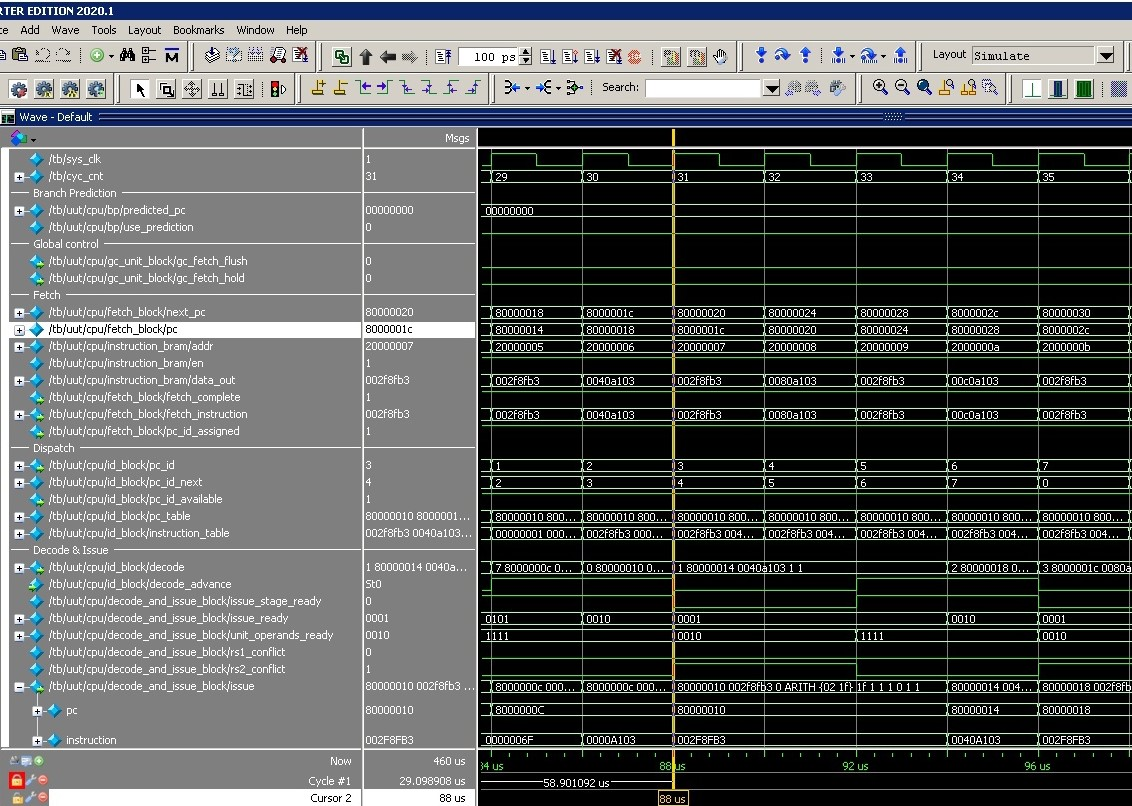
\includegraphics[scale=0.5]{images/task_2}
		\caption{Временная диаграмма выполнения стадий выборки и диспетчеризации команды с адресом 8000002с на первой итерации}
		\label{img:task_2}
	}
\end{figure}
\section{\textbf{Задание №3}}

Задание: получить снимок экрана, содержащий временную диаграмму выполнения стадии декодирования и планирования на выполнение команды с адресом 8000000с на второй итерации.

Результат представлен на рисунке \ref{img:task_3}
\begin{figure}[H]
	\captionsetup{justification=centering}
	\centering{
		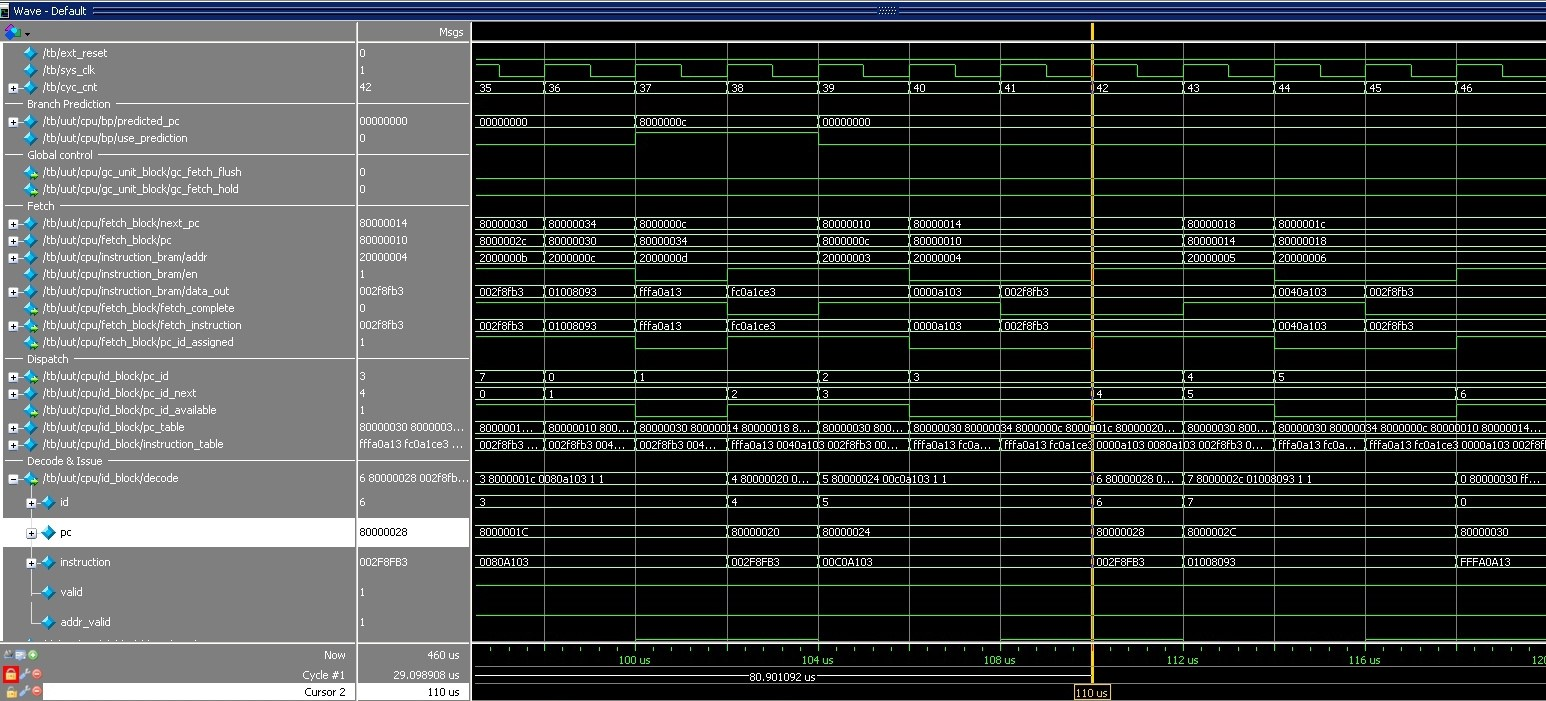
\includegraphics[scale=0.4]{images/task_3_1}
		\caption{Временная диаграмма выполнения стадии декодирования и планирования на выполнение команды с адресом 8000000с на второй итерации}
		\label{img:task_3}
	}
\end{figure}

\section{\textbf{Задание №4}}

Задание: получить снимок экрана, содержащий временную диаграмму выполнения стадии выполнения команды с адресом 80000020 на первой итерации.

Результат представлен на рисунке \ref{img:task_4}.
\begin{figure}[H]
	\captionsetup{justification=centering}
	\centering{
		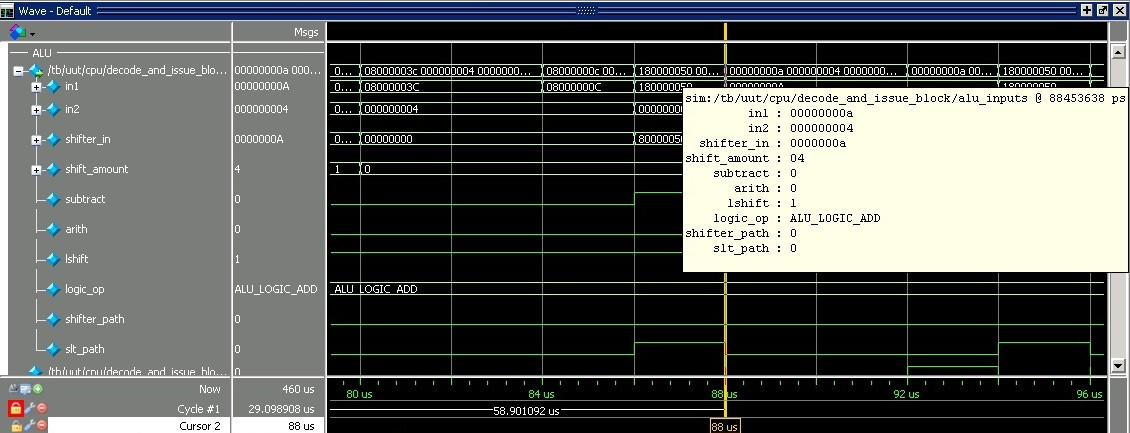
\includegraphics[scale=0.5]{images/task_4_new}
		\caption{Временная диаграмма выполнения стадии выполнения команды с адресом 80000020 на первой итерации}
		\label{img:task_4}
	}
\end{figure}

\section{\textbf{Задание №5}}
Задание: получить временную диаграмму сигналов выполнения программы индивидуального варианта. Провести оптимизацию программы путем перестановки команд для устранения конфликтов. Заполнить трассу выполнения оптимизированной программы.

\subsection{\textbf{Оптимизация}}
Конфликт происходит по регистру x20, значение которого изменяется уже после того, как выполнилась обработка над элементом массива. Предлагается сначала уменьшать число оставшихся, необработанных элементов, затем выполнять непосредственно обработку.

Код оптимизированной программы по устранению конфликтов представлен на листинге \ref{lst:new_dis}.
\begin{lstlisting}[label=lst:new_dis,caption=Исходный текст исследуемой программы]
    .section .text
	.globl _start;
	len = 9
	enroll = 1
	elem_sz = 4

_start:
	la x1, _x
	addi x20, x0, (len-1)/enroll
	lw x31, 0(x1)
	addi x1, x1, elem_sz*1
lp:
	lw x2, 0(x1)
	add x1, x1, elem_sz*enroll
	addi x20, x20, -1
	bltu x2, x31, lt
	add x31, x0, x2 #!
lt:
	bne x20, x0, lp
lp2: j lp2

	.section .data
	_x:     .4byte 0x1
	.4byte 0x2
	.4byte 0x3
	.4byte 0x4
	.4byte 0x8
	.4byte 0x6
	.4byte 0x7
	.4byte 0x5
	.4byte 0x4
\end{lstlisting}

Дизассемблированный код данной программы представлен на листинге \ref{lst:disassembler_code_new}.
\begin{lstlisting}[label=lst:disassembler_code_new, caption=Дизассемблированный код]
Disassembly of section .text:

80000000 <_start>:
80000000:       00000097            auipc   x1,0x0
80000004:       03008093            addi    x1,x1,48 # 80000030 <_x>
80000008:       00800a13            addi    x20,x0,8
8000000c:       0000af83            lw      x31,0(x1)
80000010:       00408093            addi    x1,x1,4

80000014 <lp>:
80000014:       0000a103            lw      x2,0(x1)
80000018:       00408093            addi    x1,x1,4
8000001c:       fffa0a13            addi    x20,x20,-1
80000020:       01f16463            bltu    x2,x31,80000028 <lt>
80000024:       00200fb3            add     x31,x0,x2

80000028 <lt>:
80000028:       fe0a16e3            bne     x20,x0,80000014 <lp>

8000002c <lp2>:
8000002c:       0000006f            jal     x0,8000002c <lp2>

Disassembly of section .data:

80000030 <_x>:
80000030:       0001                c.addi  x0,0
80000032:       0000                unimp
80000034:       0002                0x2
80000036:       0000                unimp
80000038:       00000003            lb      x0,0(x0) # 0 <enroll-0x1>
8000003c:       0004                c.addi4spn      x9,x2,0
8000003e:       0000                unimp
80000040:       0008                c.addi4spn      x10,x2,0
80000042:       0000                unimp
80000044:       0006                0x6
80000046:       0000                unimp
80000048:       00000007            0x7
8000004c:       0005                c.addi  x0,1
8000004e:       0000                unimp
80000050:       0004                c.addi4spn      x9,x2,0
\end{lstlisting}

Трасса исходной программы представлена на рисунке \ref{img:trace_1}.
\begin{landscape}
	\begin{figure}
		\captionsetup{justification=centering}
		\centering{
			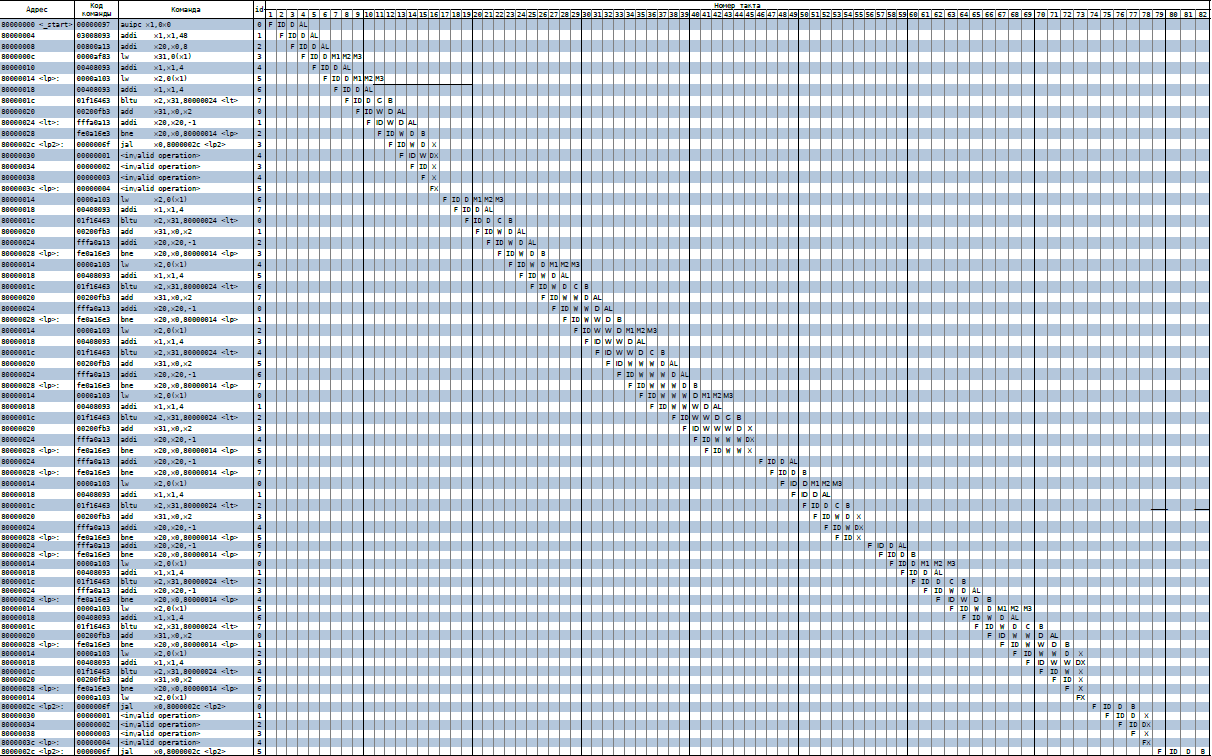
\includegraphics[scale=0.8]{images/trace_1}
			\caption{Трасса выполнения программы}
			\label{img:trace_1}
		}
	\end{figure}
\end{landscape}

Трасса оптимизированной программы представлена на рисунке \ref{img:trace_1}.
\begin{landscape}
	\begin{figure}
		\captionsetup{justification=centering}
		\centering{
			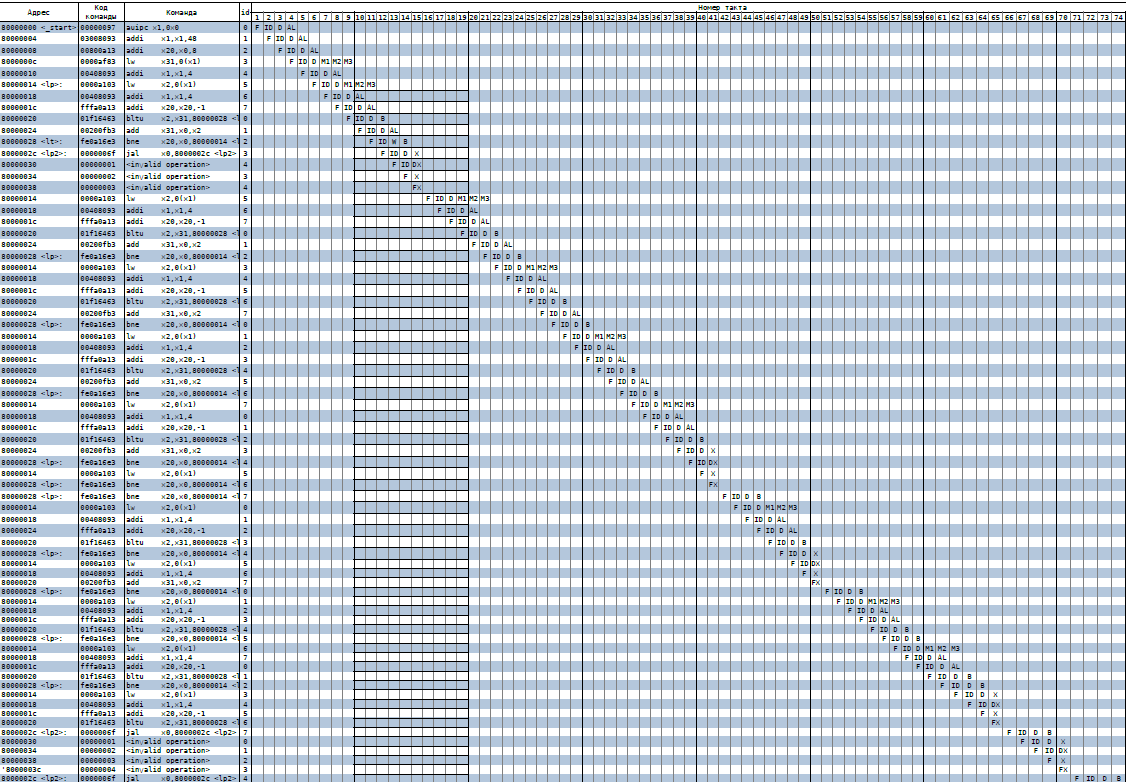
\includegraphics[scale=0.8]{images/trace_2}
			\caption{Трасса выполнения программы (оптимизированная)}
			\label{img:trace_2}
		}
	\end{figure}
\end{landscape}